\documentclass[a4paper,12pt]{report}
\usepackage{geometry}
 \geometry{
 a4paper,
 left=38mm,
 right=22mm,
 top=28mm,
 bottom=28mm,
 }

\usepackage[italian]{babel}
\usepackage[T1]{fontenc}
\usepackage{graphicx}
\usepackage[font=small]{caption}
\usepackage{color}
\usepackage{listings}
\usepackage[Glenn]{fncychap}
\usepackage{indentfirst}
\usepackage{longtable}
\usepackage{amsmath}
\usepackage{amssymb}
\usepackage{amsthm}
\usepackage{chngcntr}
\usepackage[babel]{csquotes}
\usepackage[table]{xcolor}
\usepackage{multirow}
\usepackage{gensymb}
\usepackage{pdflscape}
\usepackage{subcaption}
\usepackage{url}
\usepackage[toc,page]{appendix}
\linespread{1.5}
\counterwithout{equation}{chapter} 
\usepackage{array, booktabs}
\usepackage{comment}
\usepackage[linesnumbered, ruled]{algorithm2e}
\usepackage{xcolor}
\SetAlgorithmName{Algortimo}{Algoritmo}{Algorithm 1}
\newcommand\xqed[1]{%
	\leavevmode\unskip\penalty9999 \hbox{}\nobreak\hfill
	\quad\hbox{#1}}
\newcommand\demo{\xqed{$\square$}}
\newcommand\myworries[1]{\textcolor{red}{#1}}

\begin{document}
\author{Giulia Scoccia}
\newgeometry{
	a4paper,
	left=22mm,
	right=22mm,
	top=20mm,
	bottom=20mm,}
\begin{titlepage}
	
	\begin{center}
		\normalsize
		
		\begin{center}
			\begin{tabular}[t]{@{} l @{} c @{} r @{}}
				\parbox[c]{0.17\textwidth}{\raggedright 
\includegraphics[width=1.14in]{frontespizio/stemma2.png}}
				&
				\parbox[c]{0.7\textwidth}
				{
					\centering \bfseries
					UNIVERSIT\`A DEGLI STUDI DELL'AQUILA \\[-5pt]
					\rule{0.65\textwidth}{1pt} \\
					{\scshape Dipartimento di ingegneria e scienze dell'informazione e matematica}
				}
				&
				
				\parbox[c]{0.15\textwidth}{\raggedleft 
\includegraphics[width=1.34in]{frontespizio/disim2.png}}
			\end{tabular}
		\end{center}
		
		\bigskip \bigskip \bigskip \bigskip
				\vfil \vfil \vfil
				
		 CORSO DI LAUREA IN
		INFORMATICA
		
		\vfil \vfil \vfil		\vfil \vfil \vfil
				\vfil \vfil \vfil
		
		{\bfseries \Large
		Stima efficiente del numero di Network Motifs tramite Color-Coding e decomposizioni bilanciate}
		\vfil \vfil \vfil
				\vfil \vfil \vfil
						\vfil \vfil \vfil
								\vfil \vfil \vfil
										\vfil \vfil \vfil
										
		\makebox[\textwidth][c]{
			\begin{minipage}[t]{0.4\textwidth}
					\centering
				{\bfseries Relatore:} \\
				\underline{\hspace{\textwidth}}
				{\itshape Dott.\ Stefano Leucci} \\
				\bigskip
				\bigskip \bigskip
				{\bfseries Correlatore:} \\
				\underline{\hspace{\textwidth}}
				{\itshape Prof.\ Guido Proietti} 
				\bigskip
			\end{minipage}
			\hspace*{0.1\textwidth}
			\begin{minipage}[t]{0.4\textwidth}
				\centering
				{\bfseries Candidato:} \\
				\underline{\hspace{\textwidth}}
				{\itshape Giulia Scoccia} \\
				\bigskip
				\bigskip \bigskip
				{\bfseries Matricola:} \\
				\underline{\hspace{\textwidth}}
				{\itshape 249503} 
				\bigskip
			\end{minipage}	
		}
		\vfil \vfil \vfil	
		\rule{\textwidth}{1pt}\\
		{\scshape Anno Accademico 2019--2020}
		
	\end{center}
	
\end{titlepage}
\restoregeometry

\input{dedica}
\tableofcontents
\chapter{Introduzione}

La terapia renale di sostituzione (Renal Replacement Therapy, \textbf{RRT}) viene utilizzata sui pazienti critici in contesti di terapia intensiva che sviluppano insufficienza renale acuta (Acute Kidney Injury, \textbf{AKI}).
L'AKI è una sindrome clinica caratterizzata da un improvvisa riduzione della funzione renale risultante da un accumulo di fluidi, creatinina e urea ed altri prodotti di scarto. L'incidenza dell'AKI varia a seconda della popolazione studiata e della definizione usata. Nel 2012 le linee guida \textit{"Kidney Disease: Improving Global Outcomes"} (KDIGO) hanno definito l'AKI come un aumento del livello di creatinina sierica di 0,3 mg/dL (26,5 mmol/L) o più entro 48 ore, un livello di creatinina sierica che  aumenta di almeno 1,5 volte il valore basale nei 7 giorni precedenti o un volume di urina inferiore a 0,5 ml /kg di peso corporeo all'ora per 6 ore.
Circa il 5-7\% dei pazienti ospedalizzati sviluppa l'AKI durante la degenza ospedaliera, questa incidenza aumenta al 25\% tra i pazienti critici nell'unità di terapia intensiva\cite{tolwani2012continuous,uchino2005acute}.
È stato riportato un tasso di mortalità superiore al 50\% per i pazienti con l'AKI e insufficienza multiorgano\cite{uchino2005acute}.
In assenza di terapie farmacologiche efficaci, l'AKI viene solitamente gestita attraverso trattamenti di supporto incentrati sull'ottimizzazione dell'equilibrio dei  fluidi, sulla prevenzione o sul trattamento dei disturbi elettrolitici e acido-base, sull'aggiustamento del dosaggio dei farmaci renali ed evitando un danno renale emodinamico e nefrotossico secondario.
Oltre a queste terapie conservative, la RRT è essenzialmente l'unico metodo efficace per la gestione dei pazienti critici con l'AKI grave\cite{villa2015renal}. 
L'RRT include la dialisi (emodialisi e dialisi peritoneale), l'emofiltrazioni e la emodiafiltrazione che sono differenti metodi di filtraggio del sangue con o senza macchinari\cite{tiglis2022overview}.

Ci possono essere tre tipi di RRT:
\begin{enumerate}
	\item \textbf{Continuos renal replacement therapy (CRRT)}  è la forma  più usata in terapia intensiva. Il beneficio della CRRT per pazienti critici è che agisce lentamente (generalmente oltre 24 ore per diversi giorni) permettendo la rimozione dei fluidi e delle tossine uremiche in eccesso con meno rischi di complicazioni ipotensive\cite{karkar2019continuous}.
	\item \textbf{Intermittent renal replacement therapy (IRRT)}  eseguita per meno di 24 ore in un periodo qualunque, da due a sette volte a settimana\cite{rabindranath2007intermittent}.
	\item \textbf{Hybrid Renal Replacement Therapy  (HRRT)}  è la combinazione di entrambe le tecniche descritte in precedenza.
\end{enumerate}
Un'altro importante fattore da tenere in considerazione sono i differenti emofiltri (cioé le differenti membrane) utilizzati nelle terapie. \\
A seguire vengono presentati alcuni dei più diffusi:
\begin{itemize}
	\item \textit{\textbf{AN69/AN69ST}} è un emofiltro a membrana in poliacrilonitrile trattata in superficie, consente il fissaggio irreversibile dell'eparina alla membrana filtrante\cite{doi2017associations}. 
	
	\item \textit{\textbf{oXiris}} è una membrana dializzante modificata ricoperta con eparina, capace di rimuovere frammenti di endotossine\cite{turani2019continuous}.
	
	\item \textit{\textbf{SepteX}} caratterizzato da pori di dimensioni maggiori rispetto ai filtri convenzionali \cite{honore2013newly}.
	
\end{itemize}


La medicina evidence based, si basa su studi clinici che valutano l'efficacia dei trattamenti che poi verranno utilizzati nella pratica clinica. Spesso però risulta molto difficile validare l'efficacia dei risultati ottenuti, soprattutto se i trattamenti considerati si applicano a pazienti particolarmente critici come quelli di rianimazione, infatti è poco credibile supporre che un singolo trattamento, come ad esempio quello di purificazione ematica extracorporea possa modificare sensibilmente l'outcome di questi pazienti, che sono per loro natura estremamente complessi. 
Questo evidenzia anche come questi tipi di trattamenti non abbiano un livello di evidenza sufficiente per essere raccomandati nella pratica clinica da linee guida.

Pertanto quello che spesso avviene è che i medici utilizzino i trattamenti in maniera casuale, pensando che ci sia una ragione fisiopatologica per utilizzarli piuttosto che una direttiva che li raccomandi.

Ad esempio, si consideri il caso della purificazione ematica extracorporea mediante emoperfusione con polimixina B, per l'emoassorbimento di endotossine.
Negli ultimi quarant'anni sono stati svolti molteplici trial su questo trattamento e tutti fallimentari. In un primo trial si sono considerati tutti quei pazienti con shock settico, dopodiché si è ristretta la popolazione poiché si è notato che poteva esserci un ruolo nelle sepsi addominali, sostenute da gram negativi ed effettivamente questo poteva aver senso perché questo tipo di trattamenti va a rimuovere una specifica tossina prodotta dai batteri gram negativi.

Anche questo studio però si è rivelato fallimentare, perché solo la sottopopolazione con valori di endotossinemia elevati beneficiava effettivamente del trattamento. Questo ha senso poiché essendo proprio trattamenti per l'eliminazione delle endotossine, chiaramenti i pazienti con valori più alti andavano incontro ad una purificazione più efficace con un miglioramento clinico sensibile. 
Quindi a questo punto arruolarono i pazienti con sepsi addominali e con valori di endotossina ematica circolante per poi scoprire, anche in questo caso che la sottopopolazione di pazienti che beneficiava più di altri era quella con un determinato valore di SOFA score. 
Ossia quelli che non erano così gravi da avere un valore di SOFA molto alto e che sarebbero morti nonostante il trattamento ma neanche quelli poco gravi con un basso valore e che sarebbero sopravvissuti comunque.

Questo esempio permette di dire come l'evidence base medicine nella medicina moderna, in pazienti così complessi, con trattamenti così complessi fondamentalmente va a tentivi. 

Ed è a questo punto che entrano in gioco i registri. 
Poiché questi tipi di trial randomizzati, sono estremamente costosi e quasi sempre fallimentari, la cosa più semplice da fare a questo punto, è andare a capire e guardare cosa fa la popolazione, cosa fa il medico nella sua normale pratica clinica e, con un processo a posteriori, determinare se esistono delle sottopopolazioni di pazienti che sembrano beneficiare più di altri di questi trattamenti, così da invertire il processo di formazione delle prove. 
Quindi non identificare una popolazione, prescrivere un trattamento standard e valutare l'outcome, ma è esattamente rigirarlo cioé andare a capire quali sono i pazienti che hanno avuto esito positivo, capire come siano stati trattati. Questa identificazione dei pazienti può naturalmente essere paragonata ad una cluster analisi \cite{villa2019oxirisnet}. 

Per tutti questi motivi nel 2019, un gruppo di medici dell'Università di Firenze, ha avviato il  \textbf{Registro ARRT} (Acute Renal Replacement Therapy), con lo scopo di analizzare e studiare tutti quei casi di RRT acute.

Nel trial sono coivolti numerosi centri in tutta Italia, con circa 700 pazienti totali.

\section{Contributo della tesi}

In questo lavoro di tesi, sono stati estratti i dati dal registro ARRT tenendo traccia solo di quei pazienti sottoposti al trattamento CRRT con filtro oXiris, per cercare di ottenere il maggior numero possibile di informazioni. Prima di tutto è stata misurata la qualità dei dati e, laddove necessario, sono state applicate tecniche di data cleaning e meccanismi di miglioramento al fine di rendere il dataset risultante di qualità il più possibile accettabile. Tutto ciò per permettere in un secondo momento analisi sofisticate di Machine Learning.

Nello specifico si è cercato di clusterizzare i pazienti sulla base delle caratteristiche cliniche registrate, focalizzando le analisi su molteplici outcome di maggior interesse ai fini medici.


\section{Organizzazione del testo}

Il lavoro è suddiviso nel seguente modo.\\ 
Nel capitolo 2 viene mostrato nel dettaglio il registro ARRT. Nello specifico viene descritto come si suddivide al suo interno e per ogni sezione vengono mostrati le caratteristiche più interessanti.

Nel terzo capitolo si trovano i concetti alla base della Data Quality visti sia da un punto di vista generico che da un punto di vista medico. \\
Sempre in questo capitolo viene presentato il dataset ottenuto dal registro e vengono, inoltre, illustrate e discusse le principali criticità  riscontrate analizzando le soluzioni applicate per assicurarne una buona qualità finale.

Il capitolo 4, introduce le principali tecniche di Machine Learning utilizzate in questo lavoro e mostra i risultati sperimentali ottenuti applicando tali tecniche sul dataset.

Per concludere, nel capitolo 5 si fa un'analisi finale di tutto il lavoro svolto descrivendo dei possibili sviluppi futuri.


\chapter{Introduzione}

I Motif, anche chiamati Graphlet o Pattern, sono piccoli sottografi indotti di un grafo, la conta dei motif \`e un problema ben noto del graph mining e dell'analisi dei social network.
Dato un grafo in input, il problema richiede di contare la frequenza di tutti i graphlet di una certa taglia. 
Comprendere la distribuzione dei motif permette di avere una chiave della conoscenza delle interazioni tra le propriet\`a strutturali e i nodi del grafo.
Fa luce sul tipo di strutture locali presenti nel grafo, che possono essere usate per una miriade di analisi.
Poich\`e il conteggio dei graphlet pu\`o risultare computazionalmente impegnativo, di solito ci si accontenta di obiettivi meno ambiziosi.
Uno di questi \`e la stima della frequenza: per ogni sottografo vogliamo stimare, nel modo pi\`u accurato possibile, la sua frequenza relativa rispetto a tutti i sottografi della stessa dimensione.
Ancora meno ambiziosamente, visto che il numero di sottografi di una data dimensione cresce in modo esponenziale, si limita l'attenzione al problema della stima della frequenza relativa solo ai sottografi pi\`u ripetuti, ossia quelli che compaiono almeno una certa frazione di tempo.
Ci sono due approcci per ottenere tali stime.
Il primo \`e l'uso delle catene di Markov Monte Carlo, mentre il secondo \`e quello dell'uso del Color Coding, studi recenti mettono in luce e studiano le differenze tra i due approcci \cite{bressan2018motif}.
In questa tesi andremo a vedere il Color Coding, un'elegante tecnica randomizzata introdotta in \cite{alon1995color}, per determinare in maniera probabilistica percorsi e alberi in un grafo e pi\`u nel dettaglio una sua estensione molto interessante, l'algoritmo CC.
Questo algoritmo fornisce garanzie statistiche, forti e dimostrabili, per il problema dell'approssimazione dei conteggi esatti di graphlet, da cui le frequenze possono essere facilmente derivate, il suo utilizzo \`e molto utile applicato su grandi reti sociali \cite{bressan2018motif,bressan2019motivo}
CC si basa su due osservazioni chiave.
La prima \`e che il Color Coding pu\`o essere usato per costruire "un'urna" astratta che contiene una sotto-popolazione di tutti i k-alberi di G.
La seconda osservazione \`e che il compito di campionare k-graphlet, ossia graphlet con k nodi, pu\`o essere ridotto, con un overhead minimale, a campionare k-alberi, alberi con k nodi, dall'urna.
Si pu\`o cos\`i stimare la conta dei motif in due step: la "fase costruttiva", in cui si crea l'urna da G e la "fase di campionamento", dove si campionano i graphlet dall'urna.


\section{Contributo della tesi}

In questo lavoro di tesi, l'attenzione \`e stata concentrata sulla ricerca della frequenza di k-treelet all'interno di grafi pi\`u o meno grandi.
Per k-treelet , si intendono alberi indotti in un grafo con non k nodi.
Per effettuare tale ricerca \`e stato necessario concentrarsi sulla fase costruttiva dell'algoritmo CC.
Infatti, \`e stato visto in uno studio su una rete PPI (Protein-Protein Interaction) l'efficacia di questa fase per la ricerca della frequenza di particolari strutture biomolecolari (unicellulari e pluricelluri)\cite{alon2008biomolecular}.
La fase costruttiva, \`e descritta mediante una programmazione dinamica di tipo "top-down", \`e un processo inevitabile, che per\`o richiede un grande impiego di tempo e spazio.
Il lavoro svolto ha portato, per prima cosa ad un'implementazione, in Java.
Il programma permette la ricerca delle occorrenze dei diversi k-treelet colorati, all'interno del grafo.
Ogni albero con k nodi \`e rappresentato con una stringa binaria nella quale sono incluse tutte le informazioni, tra cui: colorazione, forma e fattore di bilanciamento ($\beta$).
I colori devono essere necessariamente k colori differenti.
Ogni albero \`e costruito in modo tale che i figli del nodo radice siano disposti in ordine non crescente.
Il fattore di bilanciamento, $\beta$, garantisce l'unicit\`a degli alberi.
Il programma mantiene tutti questi k-treelet all'interno di una tabella, insieme alle proprie occorrenze.
L'approccio alla costruzione della tabella dei treelet, a differenza dell'algoritmo originarale, \`e di tipo "bottom-up".
Per rendere pi\`u efficiente il codice si \`e ricorsi all'utilizzo di Thread.
In un secondo momento si \`e cercato di ottimizzare l'approccio utilizzato e viene introdotto il concetto di decomposizioni bilanciate di un albero.
Sfruttando queste decomposizioni si \`e riscritto il codice ottimizzato.
Anche in questo caso, in fase implementativa viene adottato un approccio "bottom-up", contrariamente a quello "top-down" adottato in fase teorica.




\section{Organizzazione del testo}

La descrizione del lavoro \`e strutturata nel seguente modo.
Nel capitolo 2 viene descritta la tecnica del color coding e il suo utilizzo per il conteggio degli alberi.
Si vedr\`a l'algoritmo CC e la sua formulazione "top-down". Si discuterà la scelta di adottare un approccio "bottom-up" per l'implementazione e i suoi vantaggi.
Nel capitolo 3 si vedranno le decomposizioni bilanciate e perch\`e aiutano per rendere l'algoritmo CC pi\`u efficiente. Anche in questo caso si discuterà sulle scelte effettuate in fase implementativa.
Nel capitolo 4 si osserveranno i dati ottenuti dalle sperimentazioni dei diversi codici.
Mentre il capitolo 5, tratter\`a le conclusione e i possibili approcci futuri.
\chapter{Color Coding}

Nel capitolo verr\`a descritta la tecnica del Color Coding utilizzata in questo studio.

La tecnica fu presentata per la prima volta nel 1995 da Alon, Yuster e Zwick \cite{alon1995color}.
In generale, dato un grafo $G = (V,E)$, il problema dell'isomorfismo dei sottografi  di $G$ \`e un problema $NP-completo$.
Il metodo del Color Coding permette di risolvere sottocasi di questo problema in tempo polinomiale.

Dati due grafi, $ G = (V,E) $ e $H = (V_H, E_H)$, i vertici $V$ di $G$, in cui verr\`a cercato un  sottografo isomorfo ad $H$, sono colorati casualmente di $k = |V_H|$ colori. Se $|V_H| = O(\log(V))$, allora tutti i vertici del sottografo di $G$ isomorfo ad $H$, se esiste, saranno colorati da colori distinti.   

Il primo algoritmo descritto, per\`o, si limitava alla ricerca di sottografi indotti in un grafo, senza farne un conteggio.
 
\`E per questo motivo che in questo capitolo si presenter\`a un'estensione dell'algoritmo descritto da Alon \cite{alon1995color}, per effettuare un conteggio dei Motif all'interno del grafo.
Dati in input un grafo $ G=(V,E) $ e un numero $ k $, per prima cosa il color coding assegna uniformemente e indipendentemente per ogni nodo di $ G $ un'etichetta in $ [k] := \{1,....,k\} $, indicato come un colore.
L'obiettivo \`e quello di conteggiare il numero di alberi colorati non indotti di $ k-nodi $ in $ G $ - chiamati $ treelet $ - i cui colori non sono ripetuti.
Questo viene fatto in maniera efficiente mediante  programmazione dinamica, una tecnica bottom-up che identifica dei sottoproblemi del problema originario, procedendo logicamente dai problemi pi\`u piccoli verso quelli pi\` grandi.




\section{Algoritmo}
\label{section1}

Qui viene descritta l'estensione dell'algoritmo del color coding che pu\`o contare e campionare treelet (non indotti) colorati uniformemnte a caso.
L'algoritmo consiste in una fase di costruzione e una fase di campionamento, in questo studio per\`o non si vede quest'ultima fase, poich\`e non rilevante ai fini di questa tesi, ma si concentra sulla prima fase.
L'algoritmo inizialmente prevede una fase di colorazione, dove per ogni nodo $ v \in V $ di $ G $ \`e assegnato un colore $ c_v $, scelto indipendentemente e uniformemente a caso da $ [k] := \{1,....,k\} $.
L'obiettivo della fase di costruzione \`e quello di creare una tabella con il conteggio dei treelet che si possono incontrare in $ G $.
Per ogni $ v $ e per ogni albero colorato $ T_C $ con $ k $ nodi, si vuole un conteggio $ c(T_C , v) $ del numero di copie di $ T_C $  in $ G $ che sono radicate in $ v $ (si noti che qui si intendono copie non indotte).
A questo fine per ogni $ v $ si inizializza $ c(T_C , v) = 1 $, dove T \`e il treelet triviale di 1 nodo e $ C = \{c_v\} $.
Successivamente si esegue una programmazione dinamica per il conteggio di treelet di dimensione $ h = 2,...,k $.
Per ogni h a turno, si considera ogni possibile albero radicato T con $ h \le k $ nodi e ogni possibile insieme di colori $ C \subseteq [k] $ con $ |C| = h $.
Poi, $ \forall v \in V $,si calcola come segue il numero $ c(T_C,v) $ di occorrenze dei treelet (non indotti) radicati in $ v $ isomorfi a $ T $ e i cui colori giacciono nell'insieme $ C $. Si divide idealmente $ T $ in due sottoalberi, unici $ T' $ e $ T'' $  radicati rispettivamente nella radice $ r $ di $ T $ e in uno dei figli di $ r $.\\
Perci\`o $ c(T_C,v) $ \`e dato come segue:
\begin{equation}\label{conta}
	c(T_c,v)=\frac{1}{\beta_T}\sum_{u\sim v}\sum_{\substack{{C',C''\subset C}\\{C'\cap C'' =0}}}c(T'_{C'},v)\cdot c(T''_{C''},u)
\end{equation}

dove $ \beta_T $ \`e una costante di normalizzazione che \'e uguale al numero di alberi di $ T $ isomorfi a $ T'' $ radicati in un figlio di $ r $. Per calcolare $ c(T_C,v) $ si passa attraverso tutti gli archi $ uv $ di $ G $, combinando i contatori di $ u $ e $ v $. La correttezza e la complessit\`a di questa costruzione, non sono trattate qui,ma vengono dimostrate in \cite{alon1995color}.

\begin{algorithm}[H]
	\SetAlgoLined
	\caption{Fase di costruzione}
 	\textbf{input} : Grafo $ G $, dimensione del treelet $ k $ \;	
 				\For{$ v $ in $ G $}{
 				$ c_v = $ viene assegnato un colore preso da [$ k $]\;
 				$ c(T_{c_v} , v) = 1 $\;
 			}	
 			\For{$ h = 2$ to $ k $}{
 				\For{$ v $ in $ G $}{
 					\ForEach{$ T : |T| = h $}{					
 						\( 	c(T_c,v)=\frac{1}{\beta_T}\sum_{u\sim v}\sum_{\substack{{C',C''\subset C}\\{C'\cap C'' =0}}}c(T'_{C'},v)\cdot c(T''_{C''},u) \)	
 					}
 				}
 			}
 			
\end{algorithm}

Come si nota, l'algoritmo itera su tutte le coppie di conteggi $ c(T'_{C'},v) $ e $ c(T''_{C''},u) $ per ogni arco $ u\sim v $ e, se $ T'_{C'}, T''_{C''}  $  possono essere unite in un albero colorato $ T_C $, allora si aggiunge $ c(T'_{C'},v) \cdots c(T''_{C''},u)  $ al conteggio $ c(T_C,v) $.
Per fare questo \`e necessaria un'operazione di ``controllo e unione'', che risulta abbastanza costosa.
Infatti, per calcolare $ c(T_C,v) $, per ogni coppia di conteggi 
Una semplice analisi ha restituito il seguente limite di complessit\`a:

\newtheorem{teorema}{Teorema}[section]
\begin{teorema}
	(\cite{bressan2018motif} \textit{Teorema 5.1} ) La fase di costruzione richiede tempo $ O(a^{k}|E|) $ e spazio $ O(a^{k}|V|) $, per un qualche $ a > 0 $.
	
\end{teorema}

La grandezza della tabella ottenuta dalla programmazione dinamica \`e il problema maggiore per l'algoritmo, infatti per $ k=6 $ e $ |V| = 5M $, sono necessari $ 45G $ di memoria.

Come si pu\'o notare, per calcolare le occorrenze di un albero $ T $ nell'algoritmo si sfrutta un approccio top-down, ossia a partire dall'albero $ T $ si identificano i due alberi $ T' $ e $ T'' $ in cui pu\`o essere scomposto e in seguito si procede al calcolo di $ c(T_C,v) $ come indicato in \ref{conta}.

In questo studio, invece, si \`e sfruttato un approccio bottom-up. Infatti, per ogni nodo $ v \in V $ di $ G $ e per ogni nodo $ u $  adiacente a $v$, si prendono due treelet colorati, rispettivamente $ T'_{C'} $ e $ T''_{C''} $, entrambi di dimensioni minori di $ h \le k $.
Se $ C' \cap C'' = 0 $ e la struttura di $ T''_{C''} $ \`e minore della struttura del pi\`u piccolo sottoalbero radicato in $ T'_{C'} $, secondo l'ordinamento totale dei treelet (vedere \ref{section 2}), allora i due treelet possono essere uniti per creare $ T_C $ le cui occorrenze saranno determinate come in \ref{conta}.

\section{Struttura dati}
\label{section 2}

	

\chapter{Decomposizioni bilanciate}

Si vuole andare a dimostrare in questo paragrafo, che dato un albero T \`e sempre possibile ricavare una scomposizione bilanciata dell'albero.
\\
Prima di poter enunciare il teorema e dimostrarlo occorre dare delle nozioni preliminari.
Innanzitutto va definito cosa si intende per scomposizione bilanciata di un albero.
\newtheorem{definizione}{Definizione}[chapter]
\newtheorem{lemma}[definizione]{Lemma}
\begin{definizione}
Sia $T_r$ un albero radicato nel nodo r , con k nodi.
Diremo che la coppia (A,B), dove  A e B sono insiemi contenenti i nodi di $T_r$, \`e una decomposizione per l'albero se:
\begin{itemize}
	\item $| A |\cup| B | = k$
	\item $A \cap B = r$.
\end{itemize}
\end{definizione}

\begin{lemma}
Affinch\`e una scomposizione risulti bilanciata dovr\`a risultare che:
\begin{equation*}
	\max{ \{|A| , |B| \} }  \le  f(k)
\end{equation*}


dove f(k) rappresenta il fattore di bilanciamento, varia in funzione al numero dei nodi dell'albero ed \`e pari a:
\begin{equation*}
f(k) = \left\lceil \frac{2}{3}  k  \right\rceil
\end{equation*}
\end{lemma}

\paragraph{Dimostrazione}\mbox{}\\\\
\begin{proof}
	Dimostrazione.....
\end{proof}

\begin{definizione}
Per ogni nodo v di un albero T, le diramazioni di T  rispetto a v, sono tutti i sottoalberi massimali, radicati nei figli di v. 
Sia $\alpha(v)$ il numero di nodi della massima diramazione di v. 

Un nodo u di un albero T con n nodi, \`e un nodo centroide se $\alpha(u)\le\frac{n}{2}$.

Il centroide di un albero non \`e necessariamente unico, infatti Jordan \cite{jordan1869assemblages}  ha dimostrato che o (i) T ha un singolo centroide v e $\alpha(v) < \frac{n}{2}$ oppure (ii) t ha due nodi centroidi (adiacenti) $v_1$ e $v_2$ tali che $\alpha(v_1) = \alpha(v_2) = \frac{n}{2}$, in questo caso il numero di nodi n \`e pari.
\end{definizione}

Esistono diversi algoritmi per la ricerca del centroide, quello da noi usato \`e l'algoritmo di Jordan che  ha una complessit\`a temporale lineare al numero di nodi O(n). \\
Il primo passo da fare \`e determinare $\alpha(v)$ $\forall v \in T$.\\
Per poter calcolare $\alpha$ $\forall v \in T$, inizialmente si effettua una visita DFS (Depth First Search) dell'albero a partire dalla radice, in modo da definire la cardinalit\`a di ogni possibile sottoalbero a partire dalla radice, procedendo su ogni suo figlio .
I sottoalberi ottenuti dai nodi foglia e dal nodo radice, sono alberi banali che avranno rispettivamente cardinalit\`a 1 e $|T|$. \\
A questo punto si pu\`o procedere con l'individuazione di $\alpha (v)$, ossia $\forall v$ della diramazione con un maggior numero di nodi.

Per farlo, si considera ogni nodo v di T e si calcola la cardinalit\`a dei sottoalberi radicati in ognuna delle sue possibili diramazioni. 
$\alpha (v)$ sar\`a il valore massimo tra tutte le quantit\`a individuate.
\\
\newtheorem{esempio}[definizione]{Esempio}
\begin{esempio}\mbox{}\\
Si prenda l’albero T in figura \ref{fig:1}.\\ 
T ha otto nodi e per ogni nodo \`e indicata la cardinalit\`a del sottoalbero radicato in esso.
\\
	\begin{figure}[htbp]
	\centering
	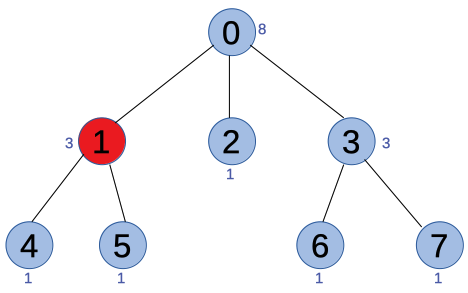
\includegraphics[width=10cm]{capitolo3/1}
	\caption{}
	\label{fig:1}
\end{figure}

Perci\`o per il nodo {\color{red} 1}, si avr\`a che:
\begin{equation*}
\alpha(1) = max {\{ |T_4| , |T_5| , (|T| - |T_1| )\}} = \max{\{1, 1, 5\} }  = 5
\end{equation*}

Dove $T_4$ rappresenta il sottoalbero di T radicato nel nodo 4, analogamente, mentre con l’ultimo valore rappresentiamo la cardinalit\`a del sottoalbero radicato in 0 e contenente tutti i nodi restanti non inclusi nel sottoalbero di T radicato in 1. 
\end{esempio}
Una volta determinato $\alpha(v)$ $\forall v \in T$, si procede alla ricerca del centroide, che sar\`a il nodo di T per cui vale la seguente disuguaglianza:
\begin{equation*}
\alpha(v) \le \left\lfloor\frac{n}{2} \right\rfloor
\end{equation*}

\paragraph{Esempio 2}\mbox{}\\
Si consideri l’albero T in figura \ref{fig:2} per la ricerca del nodo centroide.
Per prima cosa su ogni nodo di T, numerati da 0 a 10, viene calcolato $\alpha(v)$. \\\\
Quello che si otterr\`a sar\`a:

%$\alpha(0) = 6$; $\alpha(1) = 5$; $\alpha(2) = 7$; $\alpha(3) = 10$; $\alpha(4) = 7$; $\alpha(5) =  10$ $\alpha(6) = 9$; $\alpha(7) = 10$; $\alpha(8) = 10$; $\alpha(9) = 10$; $\alpha(10) = 10$.


\begin{center}
	\begin{tabular}{ c c c c c  }
		$\alpha(0) = 6$ & & $\alpha(1) = 5$ & & $\alpha(2) = 7$ \\ 
		$\alpha(3) = 10$ && $\alpha(4) = 7$ &&  $\alpha(5) =  10$ \\  
		$\alpha(6) = 9$ && $\alpha(7) = 10$ && $\alpha(8) = 10$ \\
		 $\alpha(9) = 10$ && $\alpha(10) = 10$ &&
	\end{tabular}
\end{center}
Poich\'e $ \left\lfloor\frac{n}{2} \right\rfloor = \left\lfloor \frac{11}{2} \right\rfloor = 5$, basta verificare per quale nodo v di T , vale che $\delta(v) \le \left\lfloor\frac{n}{2} \right\rfloor$.
L’unico nodo per cui tale disuguaglianza risulta vera \`e il nodo 1, infatti $5\le 5$, e sar\`a l’unico centroide dell’albero T (figura \ref{fig:3}).
	\begin{figure}[!htb]
	\begin{minipage}{0.48\textwidth}
	\centering
	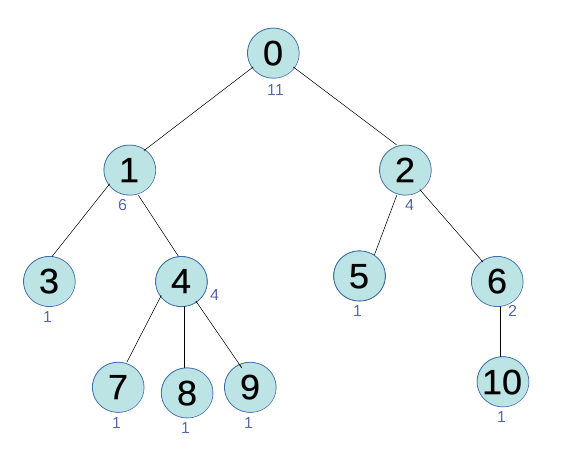
\includegraphics[width=5.26cm]{capitolo3/grafo1c}
	\caption{Rappresentazione dell'albero T}
	\label{fig:2}
	\end{minipage}\hfill
	\begin{minipage}{0.48\textwidth}
			\centering
		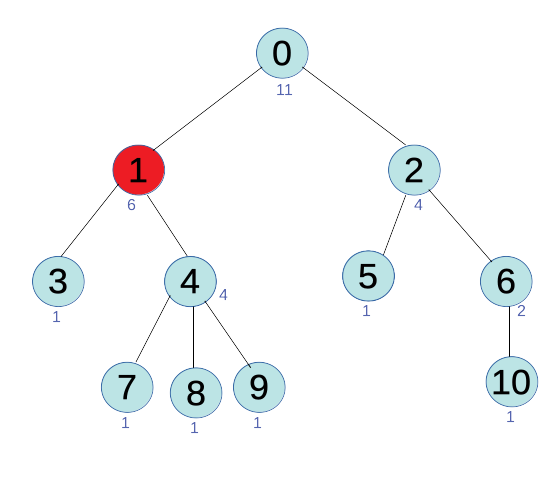
\includegraphics[width=5.8cm]{capitolo3/grafo2}
		\caption{Rappresentazione del centroide in T}
		\label{fig:3}
	\end{minipage}
\end{figure}\\
Come gia accennato l’algoritmo ha complessit\`a lineare sul numero dei nodi.
Infatti, occorre calcolare il grado di ogni nodo e successivamente verificare che ci siano le condizioni affich\`e risulti un centroide e si ha:

\begin{equation*}
\sum_{v}^{}(1 + \delta(v)) = n + \sum_{v}^{} \delta(v) = n+n-1= 2n-1 =O(n)
\end{equation*}\\
In base a tutte le nozioni illustrate in precedenza possiamo passare a ad enunciare il  teorema di seguito.

\paragraph{Teorema}\mbox{}\\
Per ogni albero T di k nodi esiste un nodo r di T , tale che l’albero $T_r$, ottenuto radicando T in r ammette una decomposizione bilanciata.

\paragraph{Dimostrazione}\mbox{}\\
Sia un albero T con pi\`u di due nodi(per $n\le2$ caso banale). \\
La prima operazione da compiere \`e l’individuazione del nodo r di T, su cui si andr\`a poi a radicare l’albero.
Banalmente, per come \`e stato definito, il nodo che si cerca, non \`e altro che  un centroide dell’albero T, quindi si applica l’algoritmo precedentemente descritto per la sua ricerca.
Una volta trovato, questo sar\`a il nuovo nodo su cui sar\`a radicato l’albero T, che da questo punto sar\`a indicato con $T_r$.
\\ 
Inoltre supponiamo, senza perdere di generalit\`a, che i sottoalberi radicati nei figli di r siano ordinati in maniera non crescente rispetto alla loro dimensione.\\
\`E possibile ottenere una scomposizione, (A,B), dei k nodi di $T_r$,  tale che un insieme, ad esempio A, contenga al massimo i $\left\lceil \frac{2}{3} \right\rceil$ dei nodi dell’albero e B il restante di essi.\\
Ovviamente questo algoritmo terminer\`a, poich\'e il numero di nodi \`e finito.
Inoltre l’insieme con il maggior numero di elementi non conterr\`a pi\`u dei $\left\lceil \frac{2}{3} \right\rceil$ del totale. \\
Per dimostrarlo si osserver\`a che A deve contenere almeno $\frac{1}{3}$ dei nodi totali. \\
Si suppone di aver inserito nell’insieme A una certa quantit\`a di elementi, sia un numero pari a $\frac{2}{3}$k. \\
Sia x il primo elemento non in A e sia i la sua posizione (figura \ref{fig:4}).
	\begin{figure}[htbp]
	\centering
	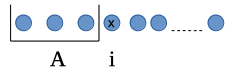
\includegraphics[width=6cm]{capitolo3/3}
	\caption{}
	\label{fig:4}
\end{figure}

Si possono verificare  due casi:
\begin{itemize}
	\item (i=2)  L’insieme A \`e formato da un unico elemento y:
		\begin{figure*}[htbp]
		\centering
		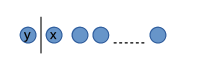
\includegraphics[width=6cm]{capitolo3/4}
			\caption{}
	\end{figure*}\\
Per come \`e costruzione di A, si avr\`a certamente che:
\\
\begin{equation}
 y + x > \frac{2}{3}k
\end{equation}
\\
Dividendo entrambi i membri di (1) per  due, si ottiene:
\\
\begin{equation}
\frac{ x + y }{2} > \frac{k}{3}  
\end{equation}
Si nota che $\frac{ x + y }{2} $ rappresenta esattamente il valore medio. \\
Dall’ordinamento dei sottoalberi di $T_r$, risulta che $y \ge x$ perci\`o si avr\`a che:
\begin{equation}
y \ge \frac{ x + y }{2} 
\end{equation}
unendo la (2) e la (3)  si ottiene:
\begin{equation*}
y > \frac{k}{3}  
\end{equation*}
\item ($i\ge3$) In A vi sono almeno due elementi. Sia s il valore ottenuto dalla loro somma 
	\begin{figure*}[htbp]
	\centering
	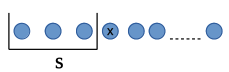
\includegraphics[width=6cm]{capitolo3/5}
		\caption{}
\end{figure*}\\
Si avr\`a che:
\begin{equation}
s+ x > \frac{2}{3}
\end{equation}
Inoltre, per costruzione:
\begin{equation}
x \le \frac{k}{3}
\end{equation}
Sottraendo la (5) alla (4), ammissibile poich\'e rispetta le regole delle disequazioni, si otterr\`a:\\
\begin{equation}
	s + x - x > \frac{2}{3} k - \frac{k}{3} \hspace{0.3cm} \text{    ossia    }\hspace{0.3cm} s > \frac{k}{3}
\end{equation}
Perci\`o gli insiemi ottenuti dalla scomposizione di $T_r$ avranno cardinalit\`a compresa tra $\frac{1}{3} k$ e $\frac{2}{3} k$, garantendo cos\`i delle decomposizioni bilanciate.\\ 
Nel caso in cui si abbiano due centroidi, la scelta su quale radicare l’albero  \`e deterministica e  viene fatta prendendo quello che, tra i due, ha un $k(v)$ minore rispetto alla relazione d’ordine precedentemente fornita.


\end{itemize}
\chapter{Conclusioni}


Nel presente lavoro di tesi è stato presentata una tecnica di realizzazione di un dataset per la clusterizzazione di pazienti critici sottoposti a trattamenti extracorporei nei reparti di terapia intesiva. 

Come descritto nell'introduzione nella medicina basata sull'evidenza la scelta di un determinato trattamento a discapito di altri non ha delle basi solide su cui basarsi,  perchè fare ricerche in merito conduce quasi sempre a studi fallimentari e con dei costi molto alti.
Negli ultimi anni si stanno sfruttando i registri medici come strumento di analisi a posteriori sui dati dei pazienti clinici, per permettere trial più efficienti ed economici. 
Pertanto un primo passo molto importante è quello di riuscire a validare i risultati fino ad oggi ottenuti sui trial con i dati ricavati dai registri.

In base a quanto ottenuto in tutto questo lavoro i risultati si dimostrano altamente promettenti. Infatti dal punto di vista medico gli esiti ottenuti già solo con la tecnica della PCA applicata sui dati del sofa score e della mortalità sembrano, ad una prima analisi, essere in linea con gli studi avvenuti negli ultimi quarant'anni. 



\section{Considerazioni finali e sviluppi futuri}

Ovviamente le più grandi criticità riscontrate sono state la grandissima eterogeneità e la mancanza corposa dei dati.
Spesso la causa di questo si può attribuire ai diversi protocolli eseguiti tra centro e centro, ma anche una scarsa educazione sulla compilazione corretta del registro.

Proprio perché ancora un pratica in sviluppo, probabilmente ancora non è chiaro il potenziale di tale sistema,infatti se le analisi mediche sui dati clusterizzati tramite K-mean validassero ulteriormente i risultati, sarebbe possibile in futuro fondere ancor meglio la data science e la medicina permettendo eventulmente misurazioni ancora più sofisticate e utili al benessere comune.



\chapter{Appendice A - Elenco sigle }




\begin{longtable}{ | c | c | } 
		\hline
		\hline
		\multicolumn{2}{|c|}{\textbf{Lista Sigle}} \\
		\hline
		\hline
		\hline
		\textbf{Sigla} & \textbf{Significato}  \\
		\hline
		\hline
		RRT & Renal Replace Therapy\\
		\hline
		CRRT & Continuous Renal Replace Therapy\\
		\hline
		IRRT & Intermitted Renal Replace Therapy\\
		\hline
		HRRT & Hybrid Renal Replace Therapy\\
		\hline
		ARRT & Acute Renal Replace Therapy\\
		\hline
		AKI & Acute Kidney Injury\\
		\hline
		KDIGO & Kindney Disease: Improving Global Outcomes\\
		\hline
		GCS & Glasgow Coma Score\\
		\hline
		ps & Pressione Sistolica\\
		\hline
		pd & Pressione Diastolica\\
		\hline
		VIS & Vasoactive Intropic Score\\
		\hline
		Tidal & Volume corrente polmonare\\
		\hline
		hct & Ematocrito\\
		\hline
		FiO2 & Frazione di ossigeno nella miscela di gas ispirati\\
		\hline
		PaO2 & Pressione parziale arteriosa dell'ossigeno\\
		\hline
		Horowitz & Rapporto $ \frac{PaO2}{FiO2} $\\
		\hline
		Qb & Flusso Sangue\\
		\hline
		Qd & Flusso liquido dialitico\\
		\hline
		Qr pre & Flusso Liquido di Replacement in Pre-Diluzione\\
		\hline
		 Qr post & Flusso Liquido di Replacement in Pre-Diluzione\\
		 \hline
		 Q-PBP & linea infusione citrato, flusso pre-blood pump\\
		 \hline
		GB & GigaByte\\
		\hline
		TB & TeraByte\\
		\hline
		PB & PetaByte\\
		\hline
		EB & EttaByte\\
		\hline
		ZB &  ZettaByte\\
		\hline
		EM & Expectation Maximization\\
		\hline
		PCA &  Principal Component Analysis\\
		\hline
		PVE & Proportion of Variance Explained \\
		\hline
				 	
\end{longtable}

\bibliography{bibliography}
\chapter*{Ringraziamenti}
\thispagestyle{empty}

Per questo lavoro ringrazio sentitamente il prof. Rossi e il dott. Manno per il supporto e la stima che hanno riposto il me. È grazie al loro aiuto e al loro supporto che oggi posso raggiungere questo traguardo così importante e ambito. 
Ringrazio inoltre il dottor Villa e il dottor Pomarè Montin dell'Università di Firenze, che mi hanno accordato la loro fiducia in questo percorso e sono sempre stati disponibili in ogni momento.

Ringrazio tutto il Cad di informatica e tutti i professori che mi hanno insegnato tanto in questi anni.

Ringrazio tutto il gruppo di Territori Aperti e di PinKamp, progetti che in questo ultimo anno mi hanno permesso di fare nuove esperienze e di incontrare tantissime persone fantastiche, in particolare devo ringraziare la prof.ssa Di Marco che ha creduto in me scegliendomi per questi lavori fantastici, penso che anche dicendo mille volte grazie non basterebbe.

Dopo i ringraziamenti "diplomatici", voglio ringraziare Andrea, Miriana, Laura, Fabio e tutti gli amici incontrati in questi anni di Università. gli sfoghi nei giorni più pesanti, le serate passate insieme e tutte le litigate giocando a qualcosa sono state un aiuto ed un relax nei momenti più duri.

Ringrazio il gruppo del pranzo/laboratorio, Andrea, Eleni, Pippo, Gianluca, Matteo, Giuseppe e tutti quelli passati nei banchi conquistati. Anche se solo per un'ora, quel tempo passato insieme è sempre stato la cosa più rilassante e piacevole della giornata.

Un grazie speciale ai Lozzi's, Angela e Daniele, per il vostro entusiasmo, la vostra pazienza e la vostra disponibilità. Quando si dice che buon sangue non mente, voi ne siete la prova. Grazie per tutto quello che siete.

Grazie ad Annaluna, perchè dietro la tua finta durezza, nascondi tanta dolcezza e riesci con poche parole a tranquillizzare chi hai di fronte.

Grazie agli Sbandieratori, che dopo tutti questi anni posso definirvi quasi una seconda famiglia. Siete rumorosi, casinari e pazzi, ma la vita senza di voi sarebbe molto più monotona e triste.

Grazie ad Alessia, Claudia e Giada, dopo più di vent'anni che ci conosciamo non penso che mi servano molte parole, perchè i gesti contano più di ogni parola.

Grazie ad Alessandro, Roberta e Paola, per le chiacchierate, le serate in tranquillità e le grandi riflessioni, anche con voi le parole sono di troppo.

Grazie alla bellissima famiglia che ho acquisito ad Avezzano, siete delle persone meravigliose, mi avete accolto da subito con tantissimo affetto e non mi avete mai fatto sentire fuori posto. Un grazie particolare ovviamente a Rossana e Giorgio, che mi avete accolto in casa vostra, senza mai farmi mancare niente. Mille volte grazie.

Grazie alla mia famiglia, che mi ha supportato durante tutto questo percorso, che mi ha appoggiato nella scelta intrapresa di rimettermi in gioco e ripartire da capo. Siete stati la mia ancora e la mia forza in molti momenti. Grazie ai miei fratelli, Giorgia e Federico e ai loro compagni, Lorenzo e Crystal, nonostante le normali litigate, so sempre che ci siete e che ci sarete. Ma grazie soprattutto a mamma e papà perchè non sarei ciò che sono senza di voi, siete le mie fondamenti e i miei pilastri e questo successo è anche vostro. 

Grazie a te Alessandro, il mio migliore amico, il mio coinquilino, il mio amore. Sei il mio consigliere più fidato e sincero. Sei la spalla sulla quale piangere quando ho bisogno, sei capaci di calmarmi e riportarmi con i piedi per terra quando serve. Non posso spiegare in poche parole tutto quello che sei, mi basta dirti che ti amo.

Grazie anche a tutti quelli che non ho nominato direttamente, ma che hanno fatto parte di questo intenso, ma bellissimo percorso. 

Infine ringrazio me stessa, per aver deciso di credere in me. Di aver investito nel mio futuro e nelle mie capacità. Di non essermi fatta demoralizzare da una società che ti vuole perfetta, perchè la perfezione non esiste. Ho capito tardi quale fosse il mio percorso, ma ringrazio ogni giorno di aver preso questa scelta, che mi auguro mi riserverà grandi soddisfazioni. 

Grazie. 




\bibliographystyle{unsrt}
\end{document}